%%%%%%%%%%%%%%%%%%%%%%%%%%%%%%%%%%%%%%%%%
% Modelo Latex para pôster do SBrT'24
%
% v1: Diego da Silva de Medeiros - IFSC
% v2: Leonardo Lira Ramalho - UFPA
%%%%%%%%%%%%%%%%%%%%%%%%%%%%%%%%%%%%%%%%%

%----------------------------------------------------------------------------------------
%	PACKAGES AND OTHER DOCUMENT CONFIGURATIONS
%----------------------------------------------------------------------------------------

\documentclass[a0,portrait]{a0poster}

\usepackage{multicol} % This is so we can have multiple columns of text side-by-side
\columnsep=100pt % This is the amount of white space between the columns in the poster
\columnseprule=3pt % This is the thickness of the black line between the columns in the poster
\usepackage{fancybox}
\usepackage[svgnames]{xcolor} % Specify colors by their 'svgnames', for a full list of all colors available see here: http://www.latextemplates.com/svgnames-colors
\usepackage{epsfig}
\usepackage{pdfpages}
\usepackage{cite}
\usepackage{color}
\usepackage{colortbl}
\usepackage[cmex10]{amsmath}
\usepackage{amssymb}
\usepackage{soul}
\usepackage{amsfonts}
%\usepackage{mathtools}
\usepackage[normalem]{ulem}
%\graphicspath{{fig/}}
%\usepackage{soul}
\usepackage{booktabs}
\usepackage{color}
\usepackage{placeins}
\usepackage{upgreek}
\usepackage[utf8]{inputenc}
\usepackage{fontspec}
\usepackage{xeCJK}

% Tikz
\usepackage{tikz}
\usetikzlibrary{shapes.geometric, arrows}

% For the table to be in the middle
\usepackage{makecell}

% set shapes
\tikzstyle{rednode} = [rectangle, rounded corners, minimum width=4cm, minimum height=2cm,
                       draw=black, fill=red!30, text width=10cm, align=center]
\tikzstyle{violetnode} = [rectangle, rounded corners, minimum width=4cm, minimum height=2cm, text centered, draw=black, fill=blue!30]
\tikzstyle{arrow} = [very thick,->,>=stealth, line width=2pt]

\setCJKmainfont{SimSun} % 或者其他你本地安装的中文字体，如 Songti SC, KaiTi, FZShuTi

\makeatletter
\renewenvironment{thebibliography}[1]
     {%
      % 不插入 section 标题
      \setlength{\parskip}{0pt}% 每条文献之间无额外间距
      \setlength{\itemsep}{0pt}% item 间距
      \setlength{\topsep}{0pt}% list 顶部空隙
      \setlength{\partopsep}{0pt}%
      \setlength{\leftmargin}{\labelwidth+\labelsep}%
      \list{\@biblabel{\@arabic\c@enumiv}}%
           {\settowidth\labelwidth{\@biblabel{#1}}%
            \usecounter{enumiv}%
            \let\p@enumiv\@empty
            \renewcommand\theenumiv{\@arabic\c@enumiv}}%
      \sloppy
      \clubpenalty4000
      \@clubpenalty \clubpenalty
      \widowpenalty4000%
      \sfcode`\.\@m
     }
     {%
      \endlist
     }
\makeatother

% 定义一个新的无编号 section 样式
\newcommand{\mysectionstar}[1]{%
  \vspace{1em} % 可调节与上文间距
  \noindent
  \tikz[baseline]{%
    \node[
      fill=SteelBlue,           % 深蓝色背景
      text width=\linewidth, % 填满整行
      align=center,        % 文字居中
      inner sep=6pt        % 内边距，可调节
    ] {\color{white}\huge\textbf{#1}};  % 白色加粗字体
  }%
  \vspace{0.0em} % 可调节与下文间距
}

\usepackage[export]{adjustbox}

%\usepackage{times} % Use the times font
%\usepackage{palatino} % Uncomment to use the Palatino font
\usepackage{epstopdf}
\usepackage{graphicx} % Required for including images
%\graphicspath{{figures/}} % Location of the graphics files
\usepackage{booktabs} % Top and bottom rules for table
\usepackage[font=small,labelfont=bf]{caption} % Required for specifying captions to tables and figures
\usepackage{amsfonts, amsmath, amsthm, amssymb} % For math fonts, symbols and environments
\usepackage{wrapfig} % Allows wrapping text around tables and figures
\usepackage[framemethod=TikZ]{mdframed}
\usepackage{lipsum}
\usepackage{titlesec} % Modify titles
%\usepackage{fontspec}
%\setmainfont{Calibri}

% set the font to be time-new roman
\usepackage{newtxtext}

% set the margin between the text and the title
\titlespacing{\section}{0pt}{1cm}{1cm}

\setlength{\parindent}{0pt}   % 段首不缩进

\newcommand{\ds}{\displaystyle}
\newcommand {\bo}[1]{\textbf{#1}}
\newcommand{\pa}[1]{\left({#1}\right)}
\newcommand{\co}[1]{\left[{#1}\right]}
\newcommand{\ch}[1]{\left\{{#1}\right\}}

% \titleformat{\section}{\color{white}\normalfont\huge\bfseries\raggedright}{\color{white}\thesection}{0.5em}{\colorbox{SteelBlue}}{}
\titleformat{\section}{\color{white}\normalfont\huge\bfseries}{\color{white}\thesection}{0.5em}{\colorbox{SteelBlue}}{}

\setlength{\columnseprule}{0pt}
\mdfdefinestyle{MyFrame}{%
	linecolor=SteelBlue,
	outerlinewidth=2pt,
	roundcorner=50pt,
	innertopmargin=\baselineskip,
	innerbottommargin=\baselineskip,
	innerrightmargin=50pt,
	innerleftmargin=50pt,
	backgroundcolor=white!50!white}
%\input{figconfig}
%\titleformat{command}[shape]{format}{label}{sep}{be %fore-code}{after-code}
\begin{document}
% \begin{mdframed}[style=MyFrame]

%----------------------------------------------------------------------------------------
%	POSTER HEADER 
%----------------------------------------------------------------------------------------

% The header is divided into two boxes:
% The first is 75% wide and houses the title, subtitle, names, university/organization and contact information
% The second is 25% wide and houses a logo for your university/organization or a photo of you
% The widths of these boxes can be easily edited to accommodate your content as you see fit
\begin{minipage}[t]{0.3\linewidth}
\raggedright
    \begin{minipage}[c]{0.2\linewidth} % logo 的子容器
      
\includegraphics[width=5cm]{logo_zjui.png}
    \end{minipage}\hspace{0.0cm}
    \begin{minipage}[c]{0.75\linewidth} % 文字信息的子容器
      \raggedright
      {\small ZJUI学院2025年暑期科研成果展} \\
      {\small 229号队伍：郑涵缤、徐嘉铭、丁昊}  \\
      {\small 指导老师：孟祥明（ZJUI 学院）} \\
      {\small \quad \quad}
    \end{minipage}
\end{minipage}
%
\begin{minipage}[c]{0.66\linewidth}
\centering
    \veryHuge \color{Navy} \textbf{One-Step Denoising with MeanFlow Model} \color{Black}\\ % Title
    \huge \color{Navy} \textbf{基于平均流模型的一步去噪}
\end{minipage}
\vspace{0.5cm}

% \vspace{3cm}
% \begin{minipage}[h]{0.98\linewidth}
% \centering \huge \color{SteelBlue} \textbf{Título do trabalho $\beta$-$\nu$-$\mu$} \color{Black}\\ % Title
% \Large \textbf{Nome S. Sobrenome\textsuperscript{1}, Nome S. Sobrenome\textsuperscript{2}, and Nome S. Sobrenome\textsuperscript{3}}\\ % Author(s)
% \normalsize \textsuperscript{1,2} Universidade, Local, Brasil\textsuperscript{1,2} and Universidade, Local, Brasil\textsuperscript{3}\\ %[-0.5cm] % University/organization
% email@email.com\textsuperscript{1}, email@email.br\textsuperscript{2} and email@email.com\textsuperscript{3}\\
% \end{minipage}
% \vspace{0.5cm} % A bit of extra whitespace between the header and poster content

%----------------------------------------------------------------------------------------

\begin{multicols}{2} % This is how many columns your poster will be broken into, a portrait poster is generally split into 2 columns


%----------------------------------------------------------------------------------------
%	ABSTRACT
%----------------------------------------------------------------------------------------

%\section*{Abstract}
\mysectionstar{Abstract}

We investigate one-step generative modeling with the recently proposed MeanFlow~\cite{geng2025mean} framework, focusing on its application for image denoising. Our method alters its initial distribution from simple distributions like Gaussian distributions to noisy images, retaining its one-step generation ability while serving the denoising purpose. We adopt the DiT architecture and conduct experiments on MNIST dataset. Results show that a single function evaluation (NFE=1) significantly reduces the noise, raising the Peak Signal-to-Noise Ratio (PSNR) from approximately 6 dB to 22.6 dB. With two evaluations (NFE=2), performance further improves to around 24 dB, whereas additional steps yield little improvement. These findings indicate that the MeanFlow structure is capable of effective denoising at minimal sampling cost, positioning it as a promising practical alternative to conventional multi-step denoising methods.

%----------------------------------------------------------------------------------------
%	Methodology
%----------------------------------------------------------------------------------------

%\section*{Methodology}\label{section:1}
\mysectionstar{Methodology}

MeanFlow Model~\cite{geng2025mean} defines the average velocity $u(z_t, r, t)$ based on the instantaneous velocity $v(z_t, t)$ in Flow Matching~\cite{lipman2023flowmatchinggenerativemodeling}. Their relationship is given by:

\begin{equation}
  u(z_t, r, t) \triangleq \frac{1}{t-r} \int_r^t v(z_\tau, \tau) \, d \tau
\end{equation}

or equivalently, using the total derivative:

\begin{equation}
  u(z_t, r, t) = v(z_t, t) - (t-r) \left[ \frac{\partial u}{\partial z_t} v(z_t, t) + \frac{\partial u}{\partial t} \right]
\end{equation}

\begin{minipage}[t]{0.45\linewidth}
  \centering
  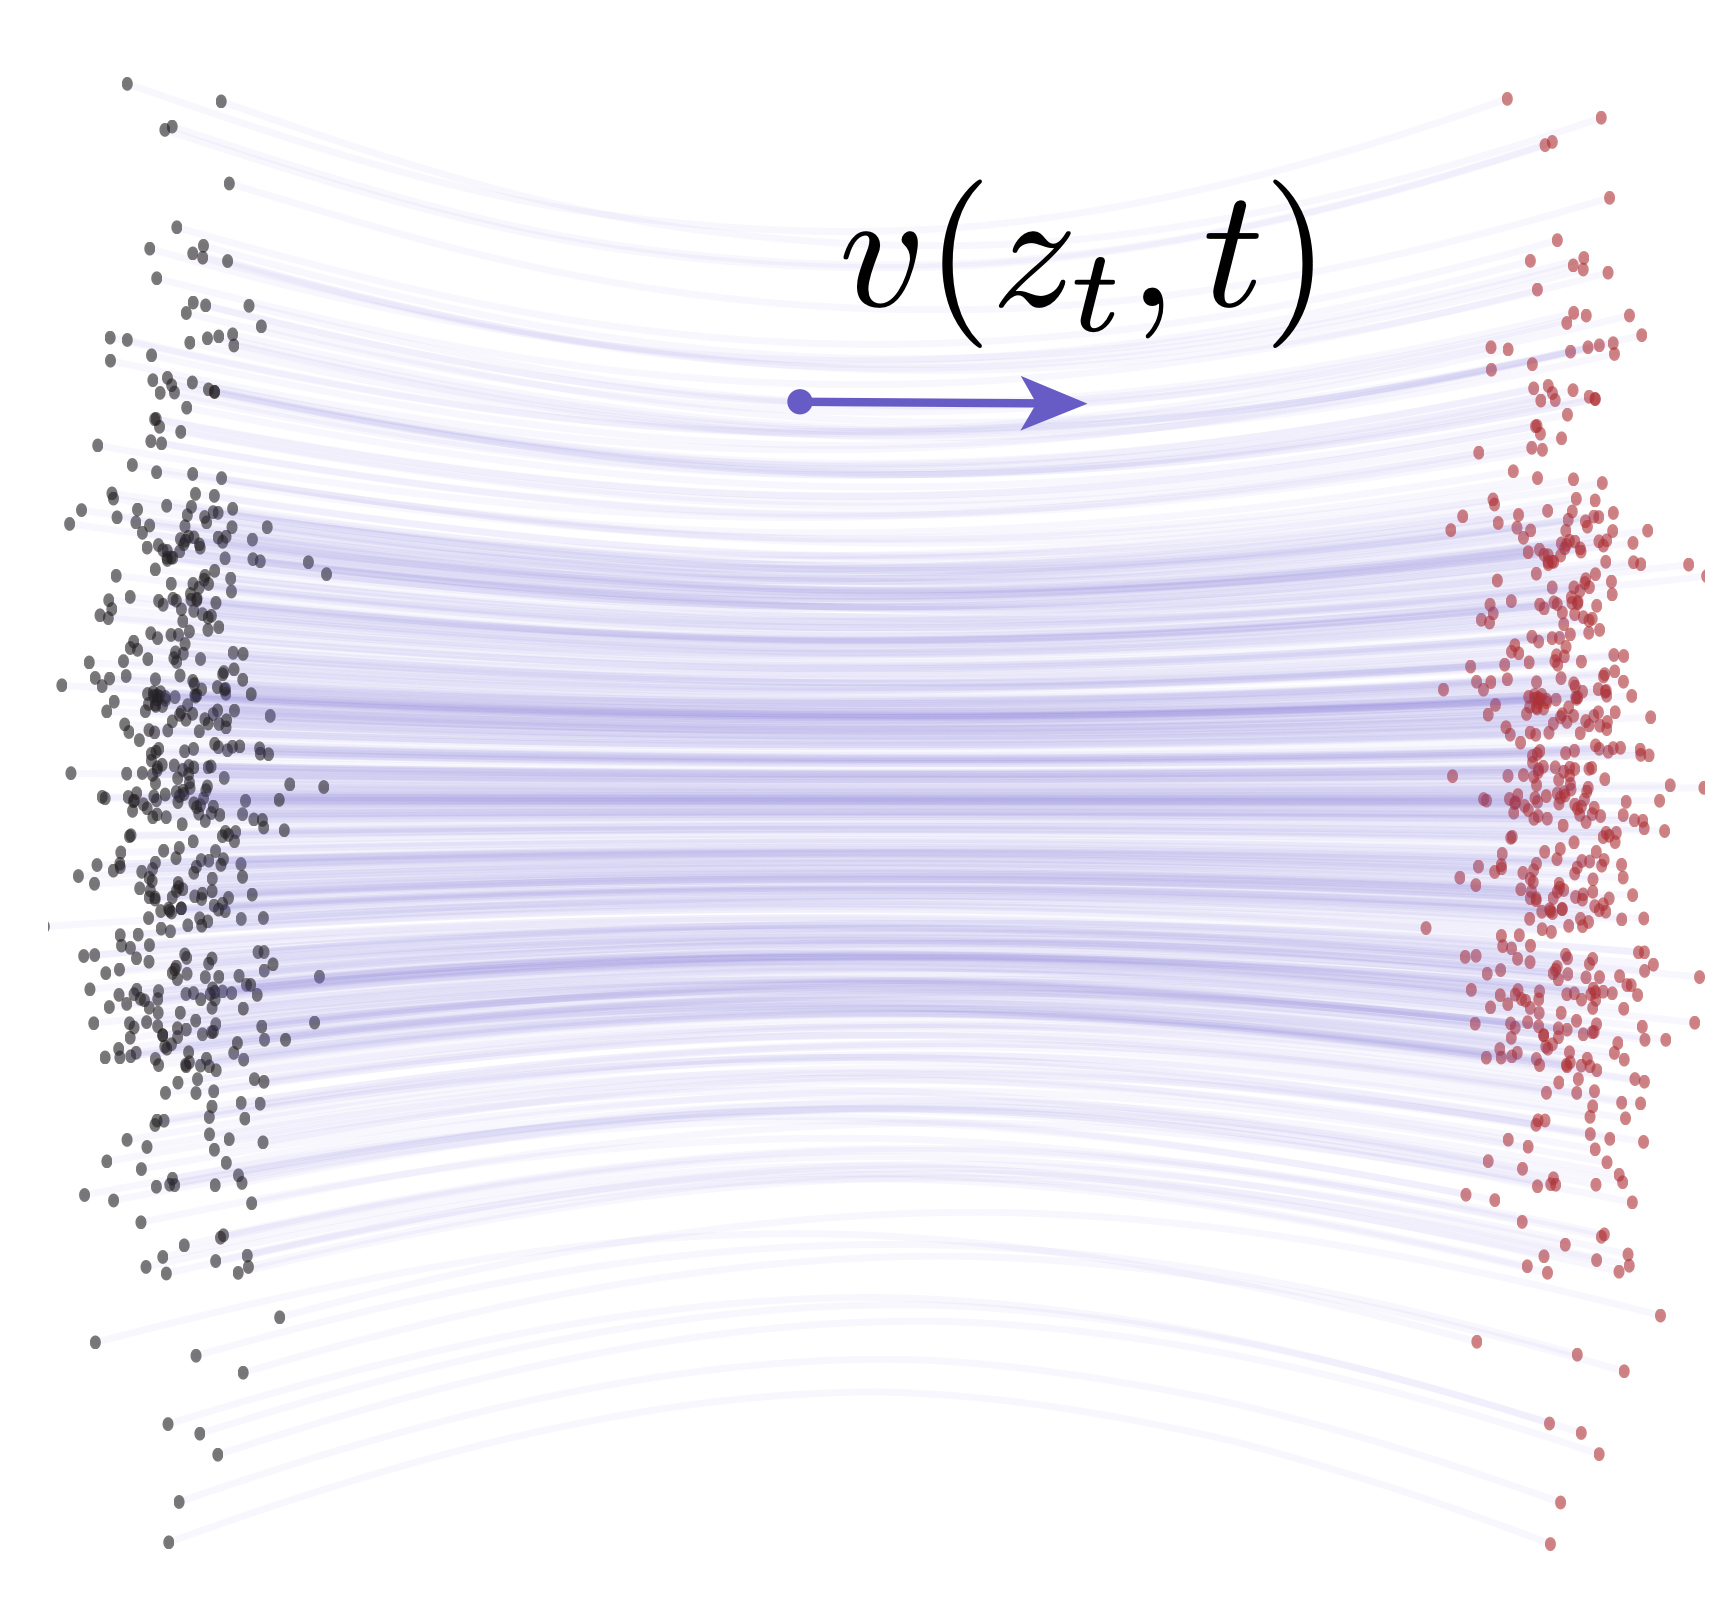
\includegraphics[width=\linewidth]{flow_matching.png} % 填满 minipage
  \captionof{figure}{Flow Matching (from~\cite{geng2025mean})}\label{fm}
\end{minipage}
\hfill
\begin{minipage}[t]{0.45\linewidth}
  \centering
  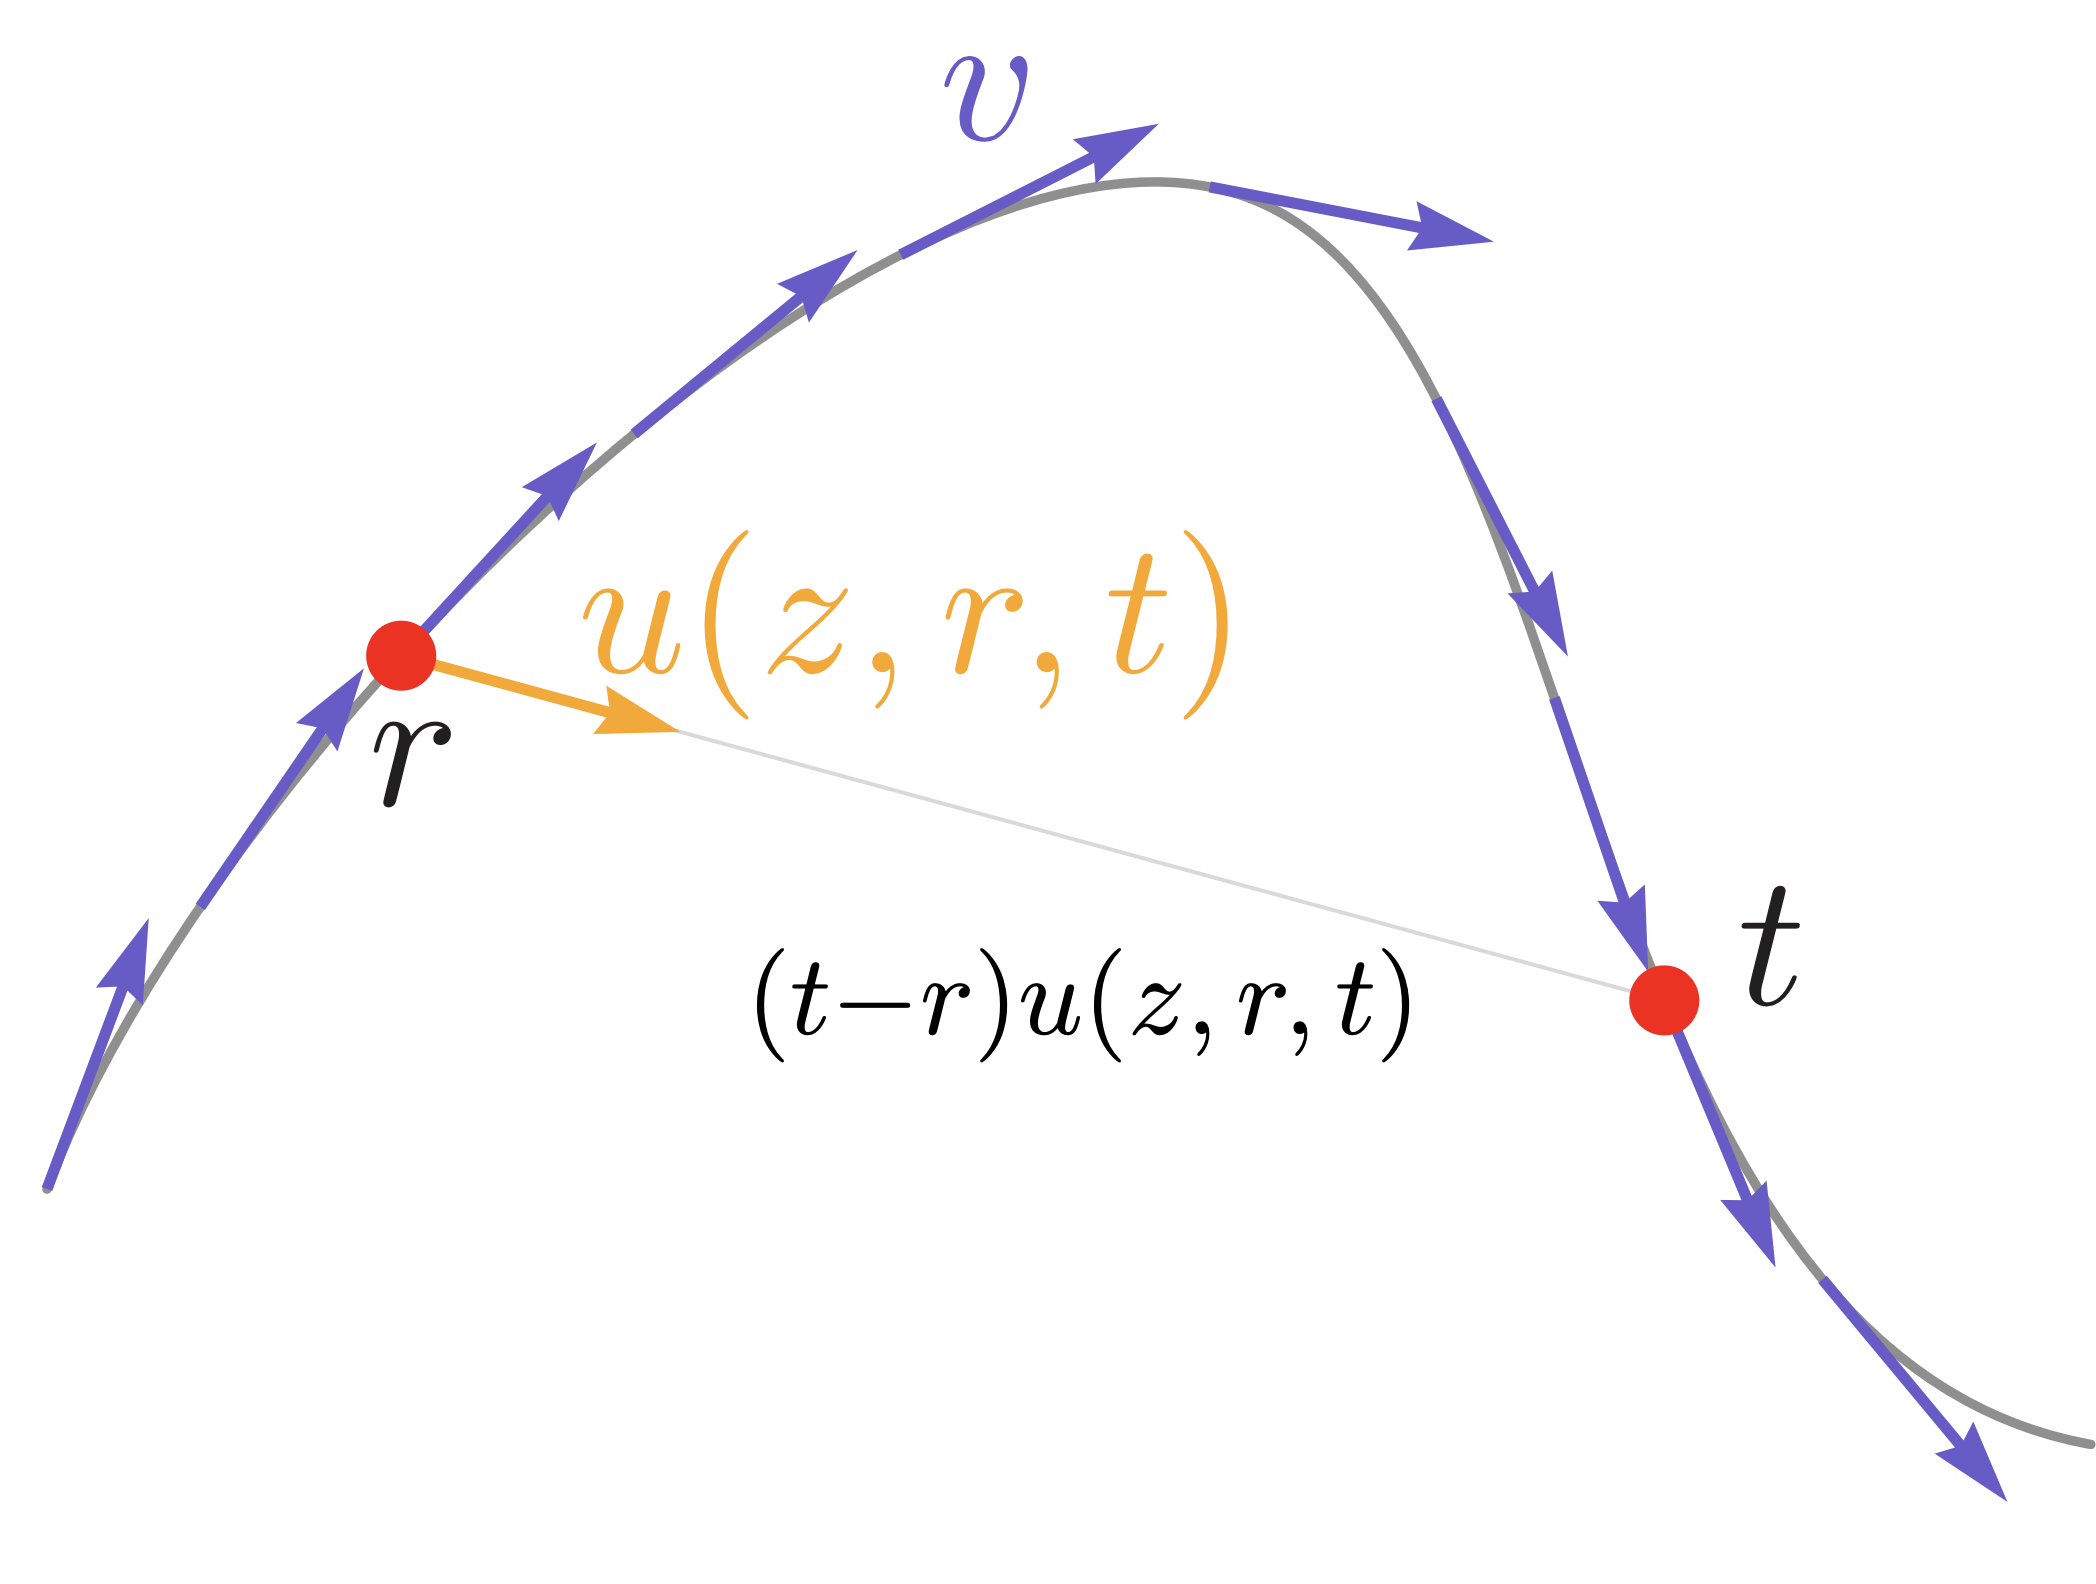
\includegraphics[width=\linewidth]{mean_flow.png} % 同样填满 minipage
  \captionof{figure}{MeanFlow (from~\cite{geng2025mean})}\label{mf}
\end{minipage}
\vspace{1cm}

Our model is built within the MeanFlow framework, incorporating classifier-free guidance (CFG)~\cite{geng2025mean} for conditional restoration. The training loss is:

\begin{equation}
  \mathcal{L^\text{cfg}_{\text{MF}}} (\theta) =
  \mathbb{E} \left[ \left\|
    u^\text{cfg}_\theta (z_t, r, t \mid c) - \text{sg} \left[ u_\text{tgt} \right]
    \right\|_2^2 \right]
\end{equation}

where the target $u_\text{tgt}$ is defined via the CFG version of the conditional instantaneous velocity $\tilde{v}_t$ and the total derivative of the average velocity:

\begin{equation}
  u_\text{tgt} = \tilde{v}_t - (t - r) \left(
  \frac{\partial u^\text{cfg}_\theta}{\partial z_t} \tilde{v}_t + \frac{\partial u^\text{cfg}_\theta}{\partial t}
  \right)
\end{equation}

The total derivative here is computed using \textbf{JVP} operation, such as \texttt{torch.func.jvp} in PyTorch, and $\tilde{v}_t$ combines the guided and unguided velocities with CFG weight $\omega$:

\begin{equation}
  \tilde{v}_t = \omega v_t + (1 - \omega) u^\text{cfg}_\theta(z_t, t, t)
\end{equation}

Finally, one-step denoising is performed via:

\begin{equation}
  z_0 = z_1 - u^\text{cfg}_\theta (z_1, 0, 1 \mid c)
\end{equation}

The training and inference procedures are illustrated in the two Pipelines below, and symbols are summarized in Table 1. \\

\begin{minipage}[c]{0.48\linewidth}
  \raggedright
  \captionof{table}{Symbols used.}
  \begin{tabular}{cc}
    \toprule
    Notation & Meaning \\
    \midrule
    $z_t$ & position at time $t$ \\
    $c$ & CFG labels \\
    $z_1$ & noisy images \\
    $x$ & clean images \\
    $t, r$ & time steps  \\
    $v_t$ & conditional instantaneous velocity \\
    $\omega$ & guidance scale for CFG \\
    $v(z_t, t)$ & instantaneous velocity at $(z_t, t)$ \\
%     $u^\text{cfg}_\theta(z_t, r, t \mid c)$ & neural network \\
    $\text{sg} \left[ \cdot \right]$ & stop gradient \\
    \bottomrule
  \end{tabular}
\end{minipage}
\hfill % 左右留空，保证两边对齐
\begin{minipage}[c]{0.48\linewidth}
  \centering
  \captionof{figure}{Pipeline for training.}
  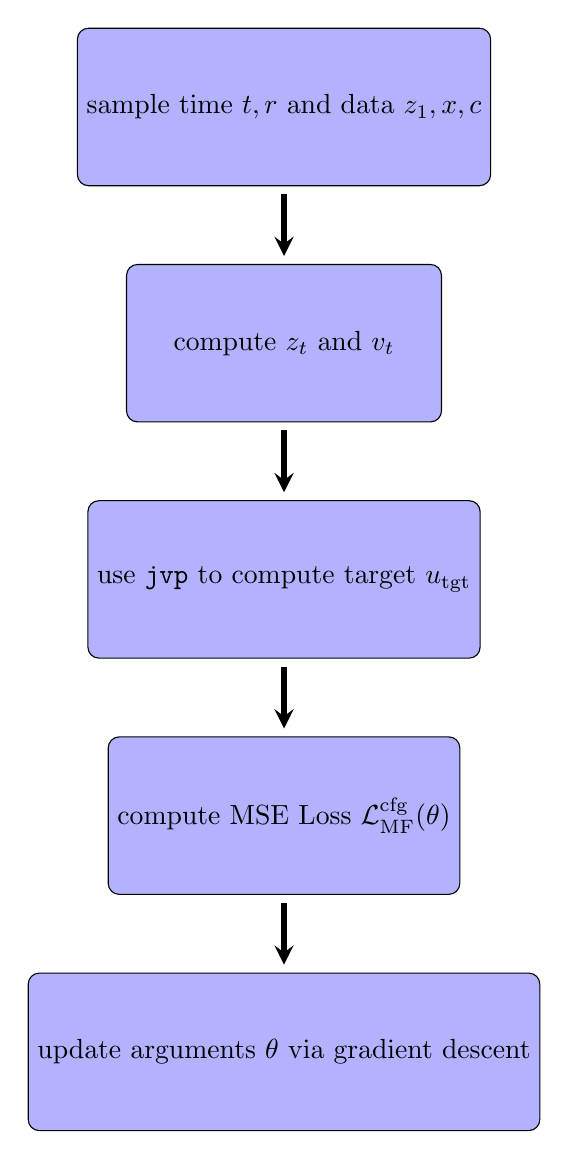
\begin{tikzpicture}[node distance=3cm]
    \node (step1) [violetnode] {sample time $t, r$ and data $z_1, x, c$};
    \node (step2) [violetnode, below of=step1] {compute $z_t$ and $v_t$};
    \node (step3) [violetnode, below of=step2] {use \texttt{jvp} to compute target $u_\text{tgt}$};
    \node (step4) [violetnode, below of=step3] {compute MSE Loss $\mathcal{L^\text{cfg}_{\text{MF}}} (\theta)$ };
    \node (step5) [violetnode, below of=step4] {update arguments $\theta$ via gradient descent};

    \draw [arrow, shorten >=1mm, shorten <=1mm] (step1) -- (step2);
    \draw [arrow, shorten >=1mm, shorten <=1mm] (step2) -- (step3);
    \draw [arrow, shorten >=1mm, shorten <=1mm] (step3) -- (step4);
    \draw [arrow, shorten >=1mm, shorten <=1mm] (step4) -- (step5);
  \end{tikzpicture}
\end{minipage}

\vspace{0.5cm}

\captionof{figure}{An overall procedure.}
\vspace{0.5cm}
\begin{tikzpicture}[node distance=12cm]
  \node (step1) [rednode] {train the model by Pipeline 1};
  \node (step2) [rednode, right of=step1] {sample noisy images $z_1$ and labels $c$ from dataset};
  \node (step3) [rednode, right of=step2] {using $z_0 = z_1 - u^\text{cfg}_\theta(z_1, 0, 1 \mid c)$ to get the result $z_0$};

  \draw [arrow, shorten >=1mm, shorten <=1mm] (step1) -- (step2);
  \draw [arrow, shorten >=1mm, shorten <=1mm] (step2) -- (step3);
\end{tikzpicture}


%
%----------------------------------------------------------------------------------------
%	Experiment
%----------------------------------------------------------------------------------------


%\section*{Experiment}\label{section2}
\mysectionstar{Experiment}

We implement our image denoising model based on the MeanFlow framework with a DiT architecture and train it using cosine annealing scheduling. As shown in Figure~\ref{psnr_over_step}, the PSNR values of 1-NFE denoising consistently improve as training progresses. Table~\ref{tab:psnr_over_step} summarizes PSNR values at different training stages, while Table~\ref{tab:psnr_over_nfe} compares denoising performance under different NFE after 300k training steps. Visual examples of the denoising results are presented in Figure~\ref{fig:mnist_img}.

\vspace{1cm}
\begin{minipage}[c]{\linewidth}
  \centering
  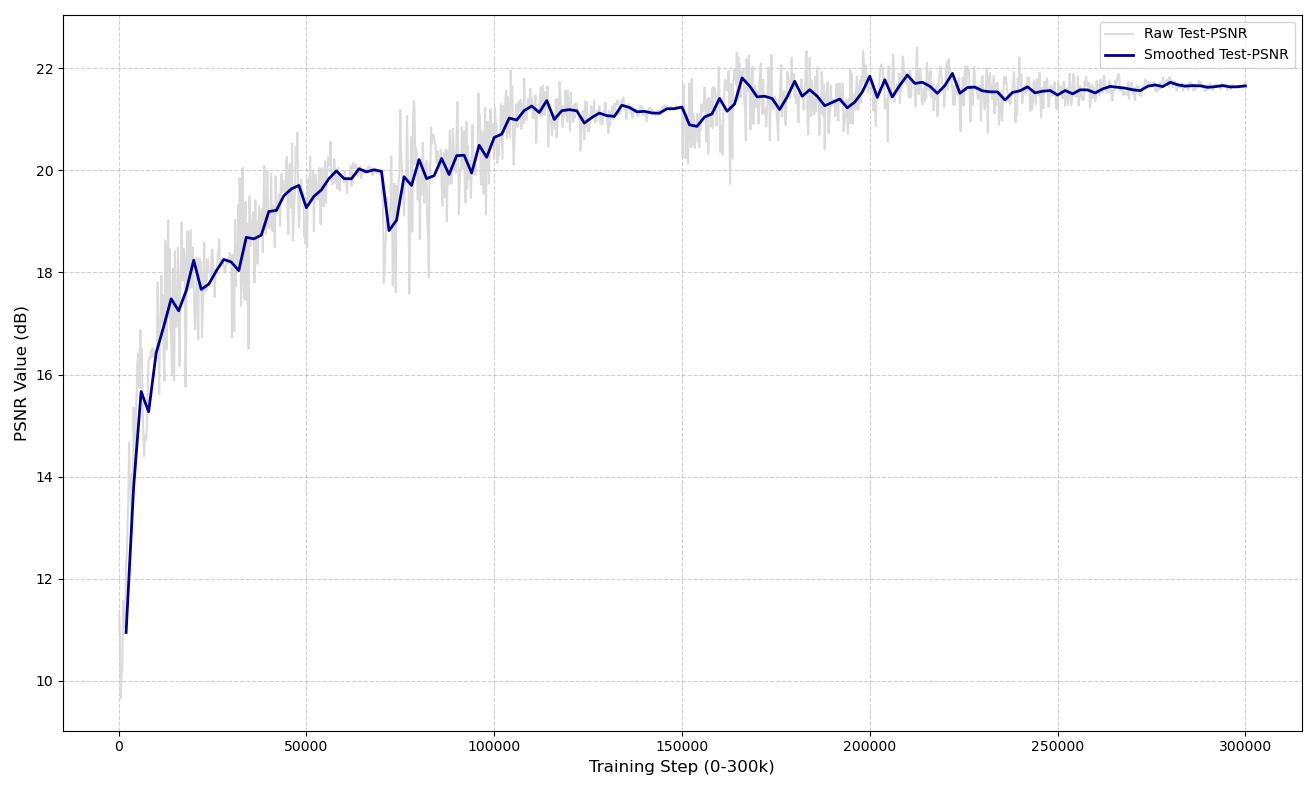
\includegraphics[width=\linewidth]{psnr_over_step.png} % 填满 minipage
  \captionof{figure}{PSNR values over training steps}\label{psnr_over_step}
\end{minipage}
\vspace{1cm}

\begin{minipage}[c]{0.48\linewidth}
  \centering
  \begin{tabular}{cc}
    \toprule
    \textbf{Images} & \textbf{PSNR (dB)} \\
    \midrule
    Noisy Input & 5.9312 \\
    2k step & 12.3043 \\
    20k step & 17.7944 \\
    100k step & 20.2236 \\
    200k step & 21.6694 \\
    300k step & 21.6807 \\
    \bottomrule
  \end{tabular}
  \captionof{table}{PSNR over training steps}\label{tab:psnr_over_step}
\end{minipage}
\hfill % 左右留空，保证两边对齐
\begin{minipage}[c]{0.48\linewidth}
  \centering
  \begin{tabular}{cc}
    \toprule
    \textbf{Images} & \textbf{PSNR (dB)} \\
    \midrule
    Noisy Input & 6.0401 \\
    1-NFE & 22.6455 \\
    2-NFE & 24.0686 \\
    3-NFE & 24.0816 \\
    4-NFE & 24.0691 \\
    5-NFE & 24.0558 \\
    \bottomrule
  \end{tabular}
  \captionof{table}{PSNR under different NFE}\label{tab:psnr_over_nfe}
\end{minipage}
\vspace{1cm}

\begin{minipage}[c]{\linewidth}
    \centering
    % 一行示例
    \noindent
    \begin{minipage}[c]{0.92\linewidth} % 图片宽度
        
\includegraphics[width=\linewidth]{mnist_img/clean.png}%
    \end{minipage}%
    \begin{minipage}[c]{0.07\linewidth} % 文字宽度
        \centering
        {\small GT}
    \end{minipage}


    \noindent
    \begin{minipage}[c]{0.92\linewidth}
        
\includegraphics[width=\linewidth]{mnist_img/noised.png}%
    \end{minipage}%
    \begin{minipage}[c]{0.07\linewidth}
        \centering
        {\small Inputs}
    \end{minipage}


    \noindent
    \begin{minipage}[c]{0.92\linewidth}
        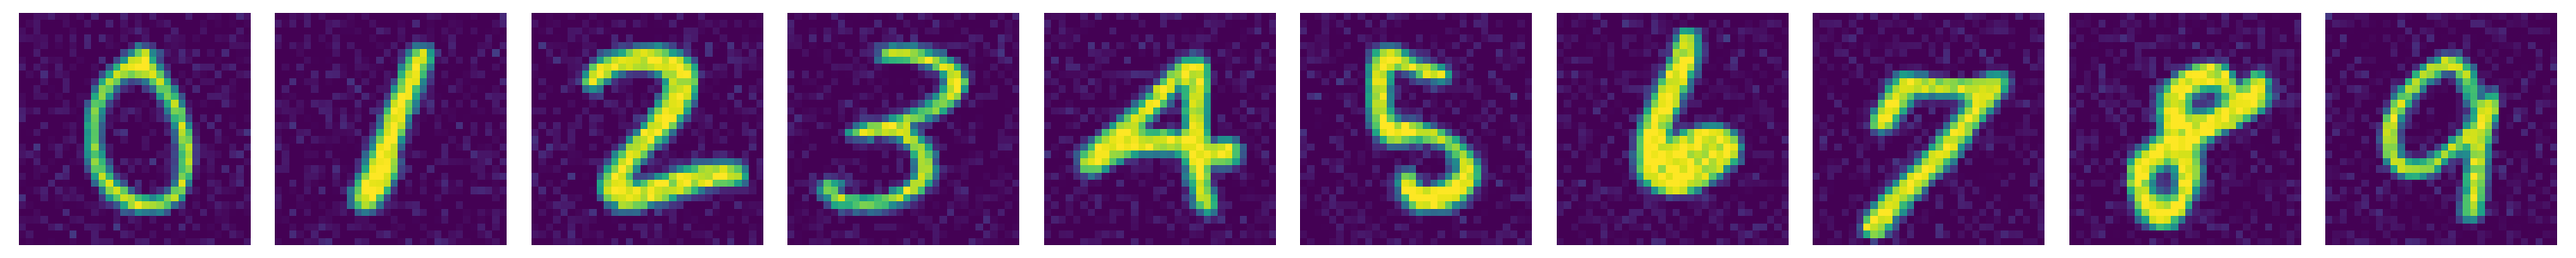
\includegraphics[width=\linewidth]{mnist_img/nfe_1.png}%
    \end{minipage}%
    \begin{minipage}[c]{0.07\linewidth}
        \centering
        {\small 1-NFE}
    \end{minipage}


    \noindent
    \begin{minipage}[c]{0.92\linewidth}
      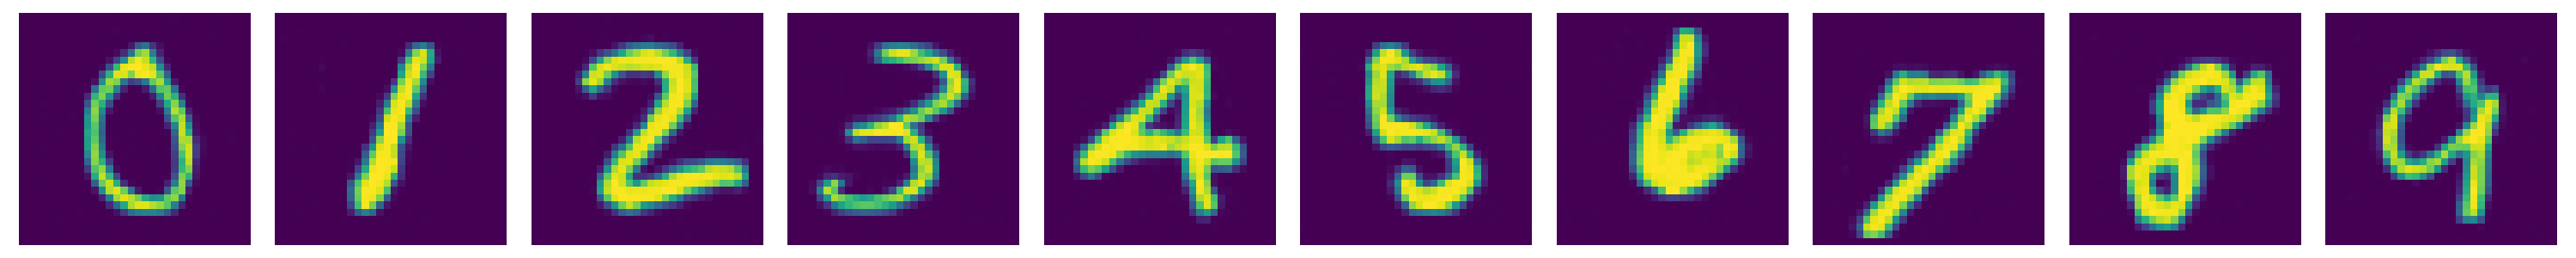
\includegraphics[width=\linewidth]{mnist_img/nfe_2.png}
    \end{minipage}
    \begin{minipage}[c]{0.07\linewidth}
      \centering
      {\small 2-NFE}
    \end{minipage}


    \noindent
    \begin{minipage}[c]{0.92\linewidth}
      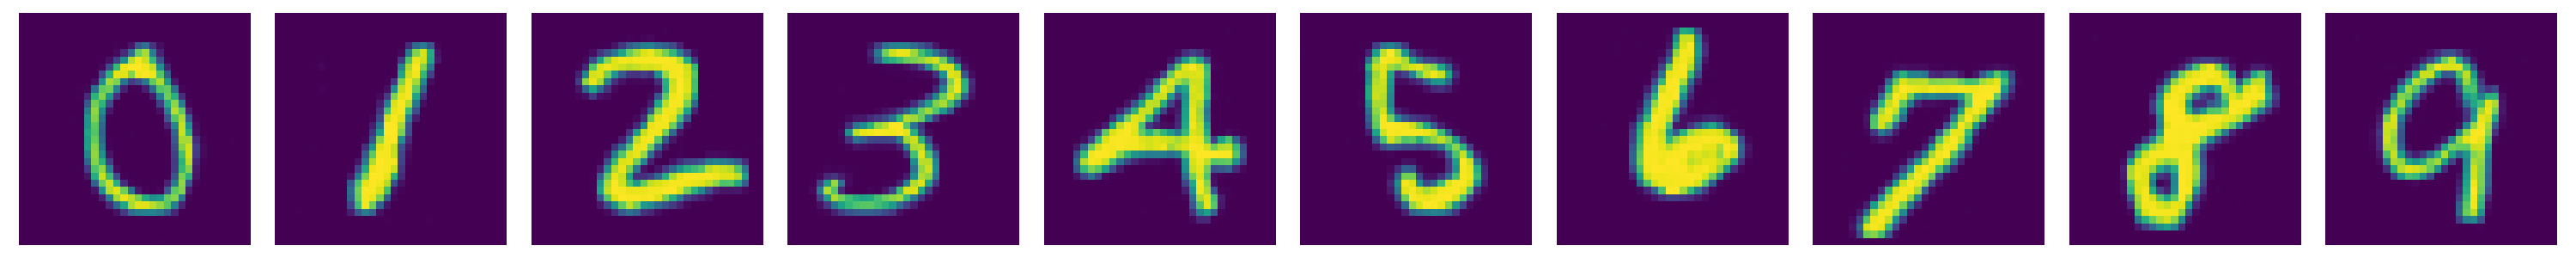
\includegraphics[width=\linewidth]{mnist_img/nfe_3.png}
    \end{minipage}
    \begin{minipage}[c]{0.07\linewidth}
      \centering
      {\small 3-NFE}
    \end{minipage}


    \noindent
    \begin{minipage}[c]{0.92\linewidth}
      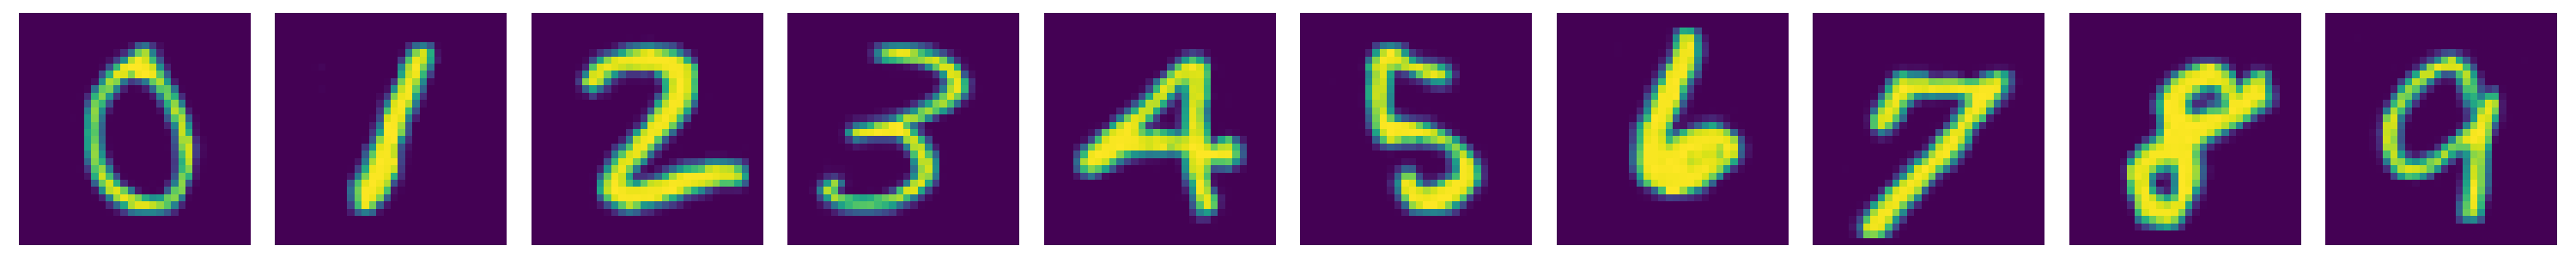
\includegraphics[width=\linewidth]{mnist_img/nfe_4.png}
    \end{minipage}
    \begin{minipage}[c]{0.07\linewidth}
      \centering
      {\small 4-NFE}
    \end{minipage}


    \noindent
    \begin{minipage}[c]{0.92\linewidth}
      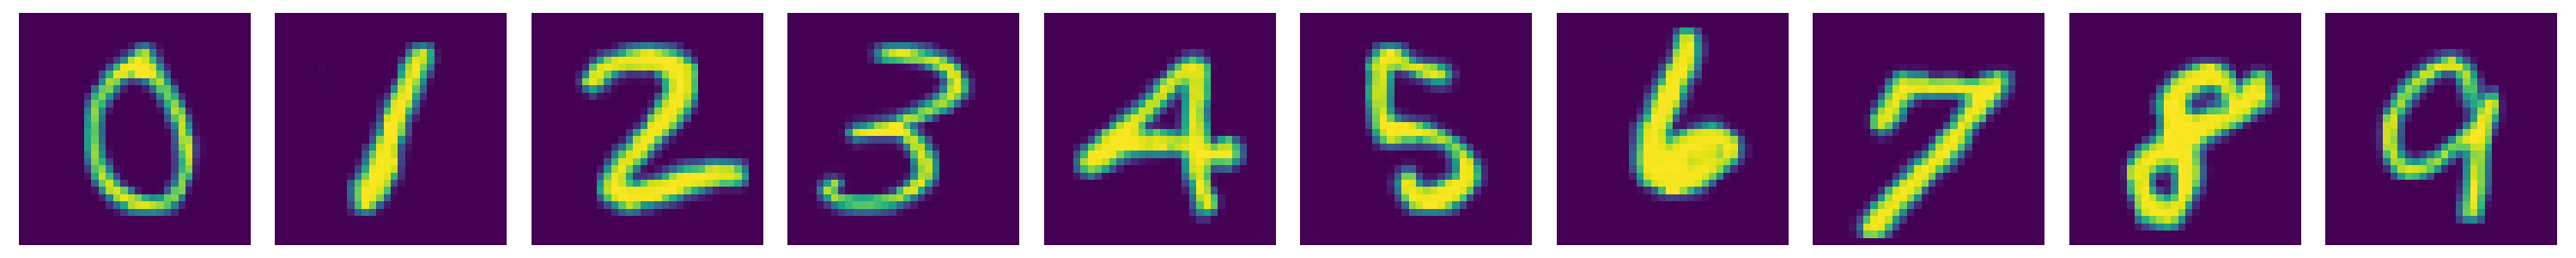
\includegraphics[width=\linewidth]{mnist_img/nfe_5.png}
    \end{minipage}
    \begin{minipage}[c]{0.07\linewidth}
      \centering
      {\small 5-NFE}
    \end{minipage}

    \captionof{figure}{Visual comparison of denoising results under different NFEs. From top to bottom: Ground Truth (clean images), Noisy Inputs, and outputs after 1 to 5 NFE denoising steps.}\label{fig:mnist_img}
\end{minipage}

%-----------------------------------------------------------------------------------------
% Conclusion
% ----------------------------------------------------------------------------------------

% \section*{Conclusion}
\mysectionstar{Conclusion}

Our experimental results demonstrate that the MeanFlow framework has considerable potential for image denoising with minimal sampling cost. While the method achieves efficient sampling, the JVP operation incurs significant computational overhead during training. Additionally, the fixed guidance scale in CFG somewhat limits its flexibility. These observations indicate that the MeanFlow architecture would benefit from further improvement, and future work could focus on developing a more computationally efficient and effective training target.


%-----------------------------------------------------------------------------------------
% Reference
% ----------------------------------------------------------------------------------------
\mysectionstar{References}

\begin{thebibliography}{99} % 开始参考文献列表环境
\bibitem{geng2025mean} Zhengyang Geng, Mingyang Deng, Xingjian Bai, et al. ``Mean Flows for One-step Generative Modeling". arXiv:2505.13447 [cs.LG], 2025.
\bibitem{lipman2023flowmatchinggenerativemodeling} Yaron Lipman, Ricky T. Q. Chen, Heli Ben-Hamu, et al. ``Flow Matching for Generative Modeling''. arXiv:2210.02747 [cs.CV], 2023.
\end{thebibliography} % 结束参考文献列表

%---------------------------------------------------
-------------------------------------
\end{multicols}

\vspace{1cm}
\begin{center}
\color{SteelBlue}{GitHub Page:} https://github.com/hanbinzheng
\end{center}
% \end{mdframed}
\end{document}
